\chapter{Conclusiones}\label{sec:conclusiones}

\paragraph{}Tras haber presentado los resultados del proyecto, vamos a terminar extrayendo
los aprendizajes y conclusiones más importantes. Para ello se va a ir repasando cada
objetivo marcado y se va a ir haciendo una valoración sobre el grado de consecución.
Se continuará hablando sobre los aprendizajes que este proyecto ha supuesto. Y por
último se van a presentar las opciones principales que se plantean como consecución al
trabajo realizado.

\section{Cumplimiento de Objetivos principales}

\paragraph{\checkmark Diseño e implementación del entorno de desarrollo:} Objetivo
cumplido, hemos construido un entorno de desarrollo totalmente funcional. Incluso se
podría considerar que finalmente han sido dos los entornos creados, uno para el entorno
de Flutter y otro para el entorno de Yocto.

\paragraph{\checkmark Diseño e implementación del ciclo de vida del desarrollo software.}
Como se ha descrito en los anteriores apartados se han diseñado las estrategias de desarrollo
y el hipotético uso de la infrestuctura necesario.

\paragraph{\checkmark Explicación del uso del entorno de desarrollo según los roles del
equipo de desarrolladores:} Objetivo cumplido, ya que se ha explicado como cada uno de
los roles interactuarán con el entorno y cuales serán las herramientas más utilizadas
en cada caso.

\paragraph{\checkmark Diseño e implementación del software de sistema:} Se ha conseguido
un software de sistema que ha resultado ser una distribución basada en linux generada
con Yocto, totalmente funcional, que permita la ejecución y uso de la aplicación embebida.

\paragraph{\checkmark Diseño e implementación de una aplicación de meteorología (frontend y
backend) de características básicas:} La aplicación que hemos llamado \emph{Rpi Weather}
es una aplicación monolítica (frontend y backend) que cumple con los casos de uso
requisitados. La elección de esta aplicación tenía intención de ser un demostrador y
como tal considero que cumple perfectamente.

\paragraph{\checkmark Procesos de testing y deployment de software manuales:}Hemo definido
sendas acciones para cada entorno y hemos conseguido hacerlas de manera manual. De esta
forma el desarrollador toma la responsabilidad de probar sus cambios antes de intentar
integrarlos.

\section{Cumplimiento de Objetivos secundarios}

\paragraph{\checkmark Análisis y justificación de las decisiones tomadas:}Considero que
a lo largo de la memoria se han ido explicando las decisiones que se han ido tomando y
que el lector ha podido comprender el por qué de las decisiones tomadas. De hecho, espero
haber podido convencer al lector de probar por su cuenta el entorno.

\paragraph{\checkmark Uso de herramientas de código abierto:} Objetivo cumplido, a continuación
desgloso un listado de todas las herramientas utilizadas así como las licencias que
utilizan.

\begin{table}[H]
    \begin{center}
    \begin{tabular}{|c|c|}
    \hline
    Yocto & GNU General Public License version 2.0 \\
    \hline
    Flutter & New BSD License \\
    \hline
    Ansible & GNU General Public License \\
    \hline
    VSCode & standard MIT license \\
    \hline
    Docker &  Docker Subscription Service Agreement* \\
    \hline
    Modelo 3D & Attribution 4.0 International (CC BY 4.0) \\
    \hline
    \end{tabular}
    \end{center}
    \caption{Ejemplo de tabla}\label{tab:table_example}
\end{table}

\paragraph{}
\emph{Aclaración licencia de docker:} Docker se distribuye bajo una licencia privativa,
no obstante, su uso es gratuito para: uso personal o proyectos de código abierto. En
caso de empresas de más de 250 personas y/o de más de 10 millones de beneficio anual,
su uso no es gratuito.

\paragraph{$\times$ Ampliación en las características demostradas con la aplicación de
meteorología:} No considero que se haya cumplido este objetivo, ya que la aplicación
no ha incluido ninguna característica adicional a las previamente marcadas.

\paragraph{\checkmark Procesos de testing y deployment de software automátizados:} Considero
que este objetivo secundario se ha conseguido, al menos parcialmente ya que aunque se
ha hecho un diseño y una propuesta de infraestuctura de testing. Además, se ha utilizado
una \emph{pipeline} de github actions para realizar los test automáticamente al subir
una nueva versión en la rama principal. La parte del deployment ha quedado sin
implementar.

\begin{figure}[H]
    \centering
    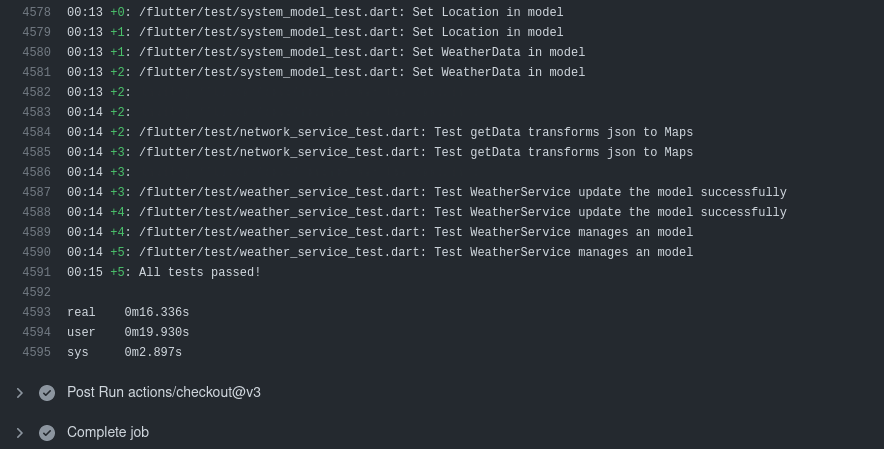
\includegraphics[width=0.85\textwidth]{imgs/github-actions-tests}
    \caption{Test pasados en una pipeline de Github Actions}
    \label{imgs:github-actions-tests}
\end{figure}

\section{Aprendizajes}

\paragraph{}A nivel técnico, puedo asegurar que la realización de este trabajo a supuesto
mucho aprendizaje para mí. Aunque he tenido experiencia previa utilizando la mayoría
de las tecnologías, nunca lo había hecho desde cero. Eso ha hecho que me diese cuenta
de los desafíos de empezar proyectos con las tecnologías utilizadas, también me ha dado
nuevas ideas, ya que al no partir de ninguna decisión previa se plantean consieraciones
que había estado ocultas.

\paragraph{}A nivel de gestión y negocio, he tenido la oportunidad de aplicar mis,
todavía, pequeños conocimientos para la toma de decisiones técnicas y ser más eficiente
o pragmático. Eso permite darte cuenta de que las decisiones técnicas sin perspectiva
de negocio pueden ser viables técnicamente pero no factibles. Al final, incluso la
gestión del tiempo propio tiene asociado un coste de oportunidad.

\paragraph{}En general, creo que puedo resumir mis aprendizajes con la siguiente lista
de consejos y afirmaciones:

\begin{itemize}
    \item Yocto es un conjunto de herramientas muy flexible para la creación de sistemas
    operativos.
    \item Yocto es muy flexible y está pensado para poder contribuir construyendo capas,
    es más fácil de reutilizar el código que con Buildroot.
    \item Bitbake es una herramienta potentísima para la gestión y configuración de tareas
    y puede tener sentido usarla más allá de Yocto.
    \item Kas es una herramienta que añade una capa de más alto nivel a bitbake. Aunque
    no es realmente necesario, resulta muy conveniente para la construcción automatizada.
    \item Kas puede ser sustituta de ``repo'', pero tiene mucha funcionalidad añadida.
    \item Aunque construir imagenes de Yocto desde cero es increiblemente lento, gestionar
    gestionar la caché sstate es vital para evitar generar lo que no cambió de generaciones
    posteriores.
    \item Usar la ccaché en Yocto también es importante cuando alguna receta falla, ya
    que la compilación de dicha receta no empieza desde el principio.
    \item No es muy necesario subir una imagen de Docker a un registry para personalizar
    un Ubuntu, al final, sólo se hace lenta la construcción, una vez construida la imagen
    lanzar contenedores es sumamente rápido.
    \item Es más cómodo de trabajar con un entorno dockerizado de lo que parece, llega
    a ser incluso transparente al usuario, ya que puedo no percibir que está trabajando
    dentro de un container.
    \item Se puede desarrollar una aplicación de escritorio para Flutter cómodamente
    usando Windows Subsystem for Linux 2 (WSL2).
    \item Flutter puede trabajar perfectamente en arquitecturas ARM en Linux, aunque
    puede haber limitaciones de rendimiento todavía.
    \item Visual Studio Code se adapta perfectamente a cada entorno de trabajo, incluso,
    ha sido utilizado para escribir la propia memoria del proyecto.

\end{itemize}

\section{Continuación del desarrollo}

\paragraph{}Un proyecto normalmente va asociado a un contrato entre empresas o a una
fecha límite, cuando esto existe, se puede consider el trabajo entregado y el proyecto
finalizado. Es posible que en ocasiones el proyecto tenga continuación con otros proyectos
que tomen como punto inicial el momento de entre del proyecto anterior o con ampliaciones
del propio proyecto. También suele haber cierta continuación a modo de soporte, ya que
rara vez un sistema debería quedar sin soporte, al menos durante un periodo de tiempo
razonable. Existen actualizaciones de dependencias, cambios de infraestuctura, cambios
de negocio, brechas de seguridad y un sin fin de asuntos que seguir atendiendo una vez
el proyecto está entregado.

\paragraph{}Dejando a un lado la continuación del mero soporte, si existiesen proyectos
de continuación bajo mi critério esto deberían ser las características que deberían
incluir:

\begin{itemize}
    \item Compatibilidad completa con sistemas operativos MacOS.
    \item Simulación del hardware con Qemu para probar el desarrollo del software de
    sistema sin necesidad del hardware.
    \item Reforzar la ciberseguridad del software de sistema, por ejemplo gestionando
    un rootfs de solo lectura y una partición para guardar la información variable.
    \item Ampliación de las capacidades de la aplicación.
        \subitem Pantallas con información más detallada.
        \subitem Previsión de las próximas horas.
        \subitem Cambio del tema a según se esté de día o de noche.
        \subitem Modo ahorro de energía.
        \subitem Registro de usuario.
    \item Upgrade del hardware a una Raspberry Pi 4.
    \item Implementación de la infraestructua en cloud o on-premises.

\end{itemize}


%las referencias a artículos se ponen con \cite,
%las referencias a glosario \gls,
%y las referencias a ecuaciones \eqref
%las referencias a imgenes, tablas o figuras o secciones
% se ponen con \ref (sólo número) o con \hyperref[sec:X]{text}
